\documentclass[12pt,titlepage]{article}
\usepackage[margin=1.25in]{geometry}
\usepackage{graphicx,amsmath,blindtext,minted}

%% Variables definition
\newcommand{\vSubject}{Object Oriented Programming}
\newcommand{\vSubtitle}{Quiz 1}
\newcommand{\vName}{Muhammad Baihaqi Aulia Asy'ari}
\newcommand{\vNIM}{2241720145}
\newcommand{\vClass}{2I}
\newcommand{\vDepartment}{Information Technology}
\newcommand{\vStudyProgram}{D4 Informatics Engineering}

%% [START] Tikz related stuff
\usepackage{tikz}
\usetikzlibrary{svg.path,calc,shapes.geometric,shapes.misc}
\tikzstyle{terminator} = [rectangle, draw, text centered, rounded corners = 1em, minimum height=2em]
\tikzstyle{preparation} = [chamfered rectangle, chamfered rectangle sep=0.75em, draw, text centered, minimum height = 2em]
\tikzstyle{process} = [rectangle, draw, text centered, minimum height=2em]
\tikzstyle{decision} = [diamond, aspect=2, draw, text centered, minimum height=2em]
\tikzstyle{data}=[trapezium, draw, text centered, trapezium left angle=60, trapezium right angle=120, minimum height=2em]
\tikzstyle{connector} = [line width=0.25mm,->]
%% [END] Tikz related stuff

%% [START] Fancy header related stuff
\usepackage{fancyhdr}
\pagestyle{fancy}
\setlength{\headheight}{15pt} % compensate fancyhdr style
\fancyhead{}
\fancyfoot{}
\fancyfoot[L]{\thepage}
\fancyfoot[R]{\textit{\vSubject - \vSubtitle}}
\renewcommand{\footrulewidth}{0.4pt}% default is 0pt, overline for footer
%% [END] Fancy header related stuff

%% [START] Custom tabular command related stuff
\usepackage{tabularx}
\newcommand{\details}[2]{
    #1 & #2  \\
}
%% [END] Custom tabular command related stuff

%% [START] Figure related stuff
\newcommand{\image}[3][1]{
    \begin{figure}[h]
        \centering
        \includegraphics[#1]{#2}
        \caption{#3}
        \label{#3}
    \end{figure}
}
%% [END] Figure related stuff

%%
\usepackage{pgf-umlcd}

\renewcommand{\umldrawcolor}{black}
\renewcommand{\umlfillcolor}{white}
%%

%% [BEGIN] Custom enumerator
\usepackage{enumitem}
%% [END] Custom enumerator

%% [BEGIN] Paragraph indent
\usepackage{indentfirst}
%% [END] Paragraph indent

\begin{document}
\begin{titlepage}
    \centering
    \vfill
    {\bfseries\LARGE
        \vSubject\\
        \vskip0.25cm
        \vSubtitle
    }
    \vfill
    
\includegraphics[width=6cm]{images/polinema-logo.png}
    \vfill
    {
        \textbf{Name}\\
        \vName\\
        \vskip0.5cm
        \textbf{NIM}\\
        \vNIM\\
        \vskip0.5cm
        \textbf{Class}\\
        \vClass\\
        \vskip0.5cm
        \textbf{Department}\\
        \vDepartment\\
        \vskip0.5cm
        \textbf{Study Program}\\
        \vStudyProgram
    }
\end{titlepage}

\newpage
\section{Quiz 1}
\subsection{Question}
\begin{enumerate}
    \item Class dan Object:
    \begin{itemize}
        \item Apa yang dimaksud dengan "class" dalam pemrograman berorientasi objek?
        \item Bagaimana Anda mendefinisikan objek dari suatu class dalam bahasa pemrograman Java?
        \item Misalkan Anda memiliki class "Barang" dalam sistem informasi inventaris. Bagaimana Anda akan membuat objek "laptop" dari class tersebut? 
    \end{itemize}
    \item Encapsulation:
        \begin{itemize}
        \item Jelaskan konsep encapsulation dalam pemrograman berorientasi objek dan mengapa hal ini penting dalam pengembangan sistem informasi inventaris barang.
        \item Dalam konteks sistem informasi inventaris, sebutkan contoh atribut (variabel) yang harus di-encapsulate dan mengapa.
    \end{itemize}
    \item Relasi Kelas:
    \begin{itemize}
        \item Apa yang dimaksud dengan relasi antara kelas dalam pemrograman berorientasi objek?
        \item Dalam sistem informasi inventaris barang, bagaimana Anda akan menggambarkan relasi antara kelas "Barang" dan kelas "Kategori"?
    \end{itemize}
    \item PBL:
    \begin{itemize}
        \item Berdasarkan kasus sistem informasi inventaris barang, coba buat sebuah class sederhana beserta atribut dan metodenya yang menggambarkan suatu entitas dalam sistem tersebut (misalnya, class "Barang").
        \item Bagaimana Anda akan menggunakan encapsulation untuk melindungi atribut - atribut dalam class tersebut?
        \item Gambarkan hierarki class atau hubungan antar class yang mungkin ada dalam sistem informasi inventaris barang di jurusan Teknologi Informasi. Berikan contoh relasi antar class (misalnya, inheritance atau association) dalam konteks tersebut.
    \end{itemize}
\end{enumerate}

\newpage
\subsection{Answer}
\begin{enumerate}
    \item Class and Object:
    \begin{itemize}
        \item Class is a frame or a template of an object. A class can have attributes and methods that represents the objects property and behaviour. 
        \item One could define an object by writing the following code:
        \begin{minted}[autogobble]{java}
            ClassName objectName = new ClassName();
        \end{minted}
        \item Object named Laptop from a class named Item:
        \begin{minted}[autogobble]{java}
            Item laptop = new Item();
        \end{minted}
    \end{itemize}
    \item Encapsulation:
    \begin{itemize}
        \item Encapsulation is a concept to isolate the class attributes so that it can only be accessed through the class setter and getter methods. Encapsulation is important because instead of the object's attributes being accessable without any rule, with the setter and getter methods the attributes can be set with a certain rule and get in a certain way the user wanted to use.
        \item An attribute that could be encapsulate in that case might be the amount of item stored since there could be a limit to the amount of item the object can store. 
    \end{itemize}
    \item Class Relation:
    \begin{itemize}
        \item Class relation is a concept of a class using, having, or inheriting a class.
        \item Here is a UML diagram that represents the relation between the class "Item" and the class "Category".
        \begin{center}
            \includegraphics[width=.15\textwidth]{images/figures/fig1.drawio.png}
        \end{center}
    \end{itemize}
    \newpage
    \item Project Based Learning:
    \begin{itemize}
        \item -
        \begin{center}
            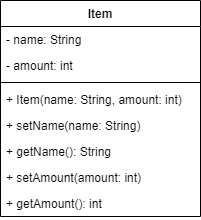
\includegraphics[width=.3\textwidth]{images/figures/fig2.drawio.png}
        \end{center}
        \item To protect the attribute the class has a setter and getter methods.
        \item -
        \begin{center}
            \includegraphics[width=.3\textwidth]{images/figures/fig3.drawio.png}
        \end{center}
    \end{itemize}
\end{enumerate}

\end{document}